%texexptitled======================================================================
% lab1-gcd
%-----------------------------------------------------------------------
%

\documentclass[11pt]{article}

% Package includes

\usepackage{graphicx}
\usepackage{color}
\usepackage{comment}
\usepackage{multirow}
\usepackage{askmaps}
\usepackage{amssymb}
\usepackage{amsmath}
\usepackage{tikz}
\usepackage{circuitikzgit}
\usetikzlibrary{arrows, positioning, shapes.geometric, circuits.logic.US}
\tikzstyle{line}=[draw]
\tikzstyle{arrow}=[draw, -latex]

% Wrap long URLs with hyphens
\PassOptionsToPackage{hyphens}{url}\usepackage{hyperref}
\usepackage{pdftexcmds}
\usepackage{upquote}
\usepackage{textcomp}
\usepackage{minted}
\usepackage[listings]{tcolorbox}
\usepackage{enumerate}
\usepackage{enumitem}
\usepackage{mathtools}
\DeclarePairedDelimiter{\ceil}{\Big\lceil}{\Big\rceil}

\tcbset{
texexp/.style={colframe=black, colback=lightgray!15,
         coltitle=white,
         fonttitle=\small\sffamily\bfseries, fontupper=\small, fontlower=\small},
     example/.style 2 args={texexp,
title={Question \thetcbcounter: #1},label={#2}},
}

\newtcolorbox{texexp}[1]{texexp}
\newtcolorbox[auto counter]{texexptitled}[3][]{%
example={#2}{#3},#1}

\setlength{\topmargin}{-0.5in}
\setlength{\textheight}{9in}
\setlength{\oddsidemargin}{0in}
\setlength{\evensidemargin}{0in}
\setlength{\textwidth}{6.5in}

% Useful macros

\newcommand{\note}[1]{{\bf [ NOTE: #1 ]}}
\newcommand{\fixme}[1]{{\bf [ FIXME: #1 ]}}
\newcommand{\wunits}[2]{\mbox{#1\,#2}}
\newcommand{\um}{\mbox{$\mu$m}}
\newcommand{\xum}[1]{\wunits{#1}{\um}}
\newcommand{\by}[2]{\mbox{#1$\times$#2}}
\newcommand{\byby}[3]{\mbox{#1$\times$#2$\times$#3}}


\newenvironment{tightlist}
{\begin{itemize}
 \setlength{\parsep}{0pt}
 \setlength{\itemsep}{-2pt}}
{\end{itemize}}

\newenvironment{titledtightlist}[1]
{\noindent
 ~~\textbf{#1}
 \begin{itemize}
 \setlength{\parsep}{0pt}
 \setlength{\itemsep}{-2pt}}
{\end{itemize}}

% Change spacing before and after section headers

\makeatletter
\renewcommand{\section}
{\@startsection {section}{1}{0pt}
 {-2ex}
 {1ex}
 {\bfseries\Large}}
\makeatother

\makeatletter
\renewcommand{\subsection}
{\@startsection {subsection}{1}{0pt}
 {-1ex}
 {0.5ex}
 {\bfseries\normalsize}}
\makeatother

% Reduce likelihood of a single line at the top/bottom of page

\clubpenalty=2000
\widowpenalty=2000

% Other commands and parameters

\pagestyle{myheadings}
\setlength{\parindent}{0in}
\setlength{\parskip}{10pt}

% Commands for register format figures.

\newcommand{\instbit}[1]{\mbox{\scriptsize #1}}
\newcommand{\instbitrange}[2]{\instbit{#1} \hfill \instbit{#2}}

\graphicspath{{./figs/}}


%-----------------------------------------------------------------------
% Document
%-----------------------------------------------------------------------

\begin{document}
\def\PYZsq{\textquotesingle}

\renewcommand{\arraystretch}{1.5}

\newcommand{\headertext}{EE240B HW3}
\renewcommand{\thesubsection}{\thesection.\alph{subsection}}

\newcommand{\Ohms}{\text{ }\Omega}
\newcommand{\MOhms}{\text{ M}\Omega}

\newcommand{\VNoise}{\frac{\text{V}}{\sqrt{\text{Hz}}}}
\newcommand{\nVNoise}{\frac{\text{nV}}{\sqrt{\text{Hz}}}}

\title{\vspace{-0.4in}\Large \bf \headertext \vspace{-0.1in}}
\author{Vighnesh Iyer}

\date{\today}
\maketitle

\markboth{\headertext}{\headertext}
\thispagestyle{empty}

\section{Amplifier Noise}
{\color{blue}For the circuit below calculate the transconductance $g_m$ that minimizes the minimum detectable signal (when $I_{in}$ equals to input-referred current noise) as a function of $\gamma$, $\omega_T$, and $C_s$. In the plot of MDS vs $g_m$, comment briefly on why there is a minimum and how the slope relates to $g_m$. Consider $C_{gs}$ and ignore $C_{gd}$.}

\begin{figure}[H]
  \centering
  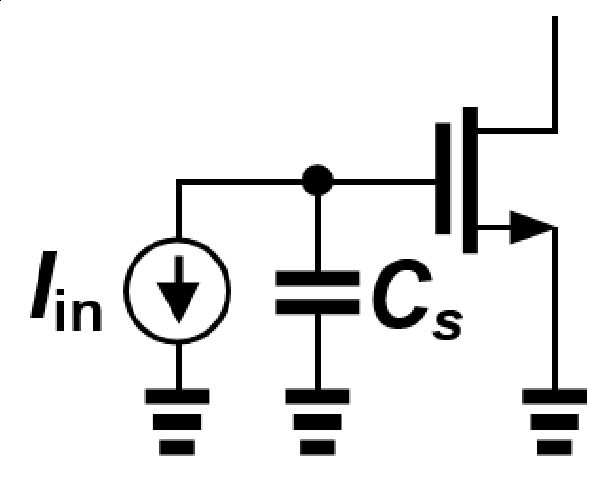
\includegraphics[width=0.2\textwidth]{figs/problem1.png}
\end{figure}

I think the answer is just that, to first order, the MDS is independent of $g_m$; this is because $\omega_T = \frac{g_m}{C_s}$ and $\omega_T$ is a process and bias constant. Therefore any increase in $C_s$ would also necessitate a proportional increase in $g_m$. Notice that the output noise caused by a current noise at the input is $\overline{i_s^2} \left( \frac{\omega_T}{\omega} \right)^2$ which is a constant!

The solution doesn't make sense. Firstly the 2 expressions given for $\overline{i^2_{out}}$ aren't equal; they are off by a factor of 4.

But that shouldn't change the optimal $g_m$ anyways. Indeed if you differentiate and set to 0 the expression in the solution, the solution $g_{m,opt} = C_s \omega_T$ is what comes out, but that just equals $g_m$ again! How is it legitimate to differentiate the expression in the solution wrt $g_m$ if $\omega_T$ itself can be written in terms of $g_m$?

\section{Amplifier Design}
\begin{enumerate}[label=(\alph*)]
  \item {\color{blue}What is the total noise at the output of the common-source-common-drain cascade shown below? Ignore flicker noise, $r_o$, and capacitor except those drawn in the diagram. You should provide your answer in terms of $kT, C_1, C_2, \gamma, A_{v1}, A_{v2}, \omega_{p1}, \omega_{p2}$. $A_{v1,v2}$ and $\omega_{p1,p2}$ are the low-frequency voltage gains and dominant poles of the two stages.}

  \begin{figure}[H]
    \centering
    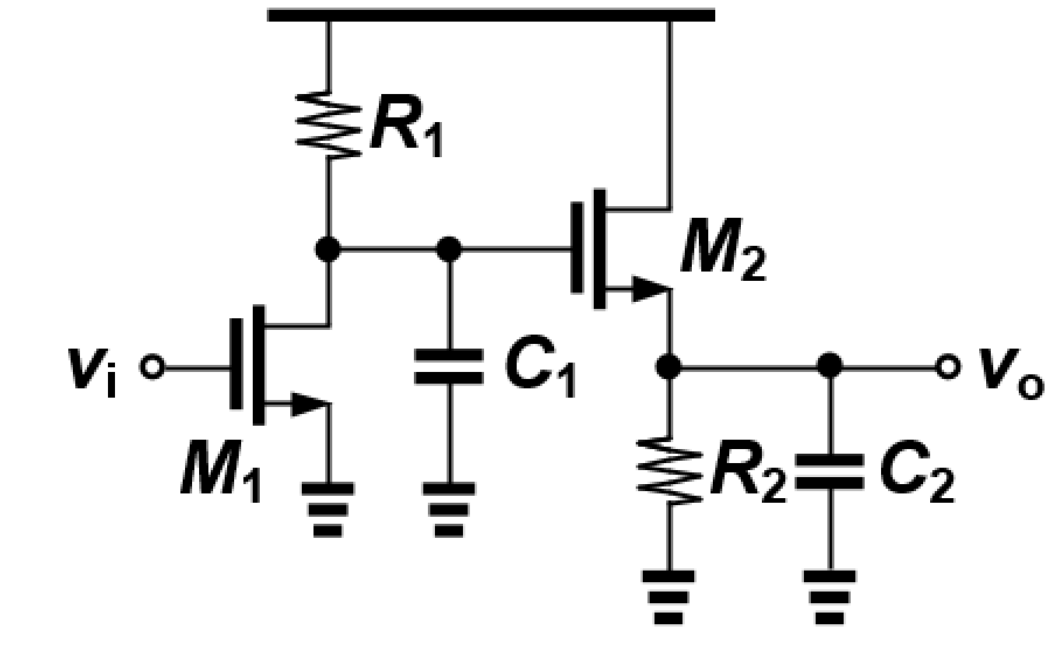
\includegraphics[width=0.4\textwidth]{figs/problem2.png}
  \end{figure}
  \begin{align*}
    \overline{v_{n,o}^2} &= \underbrace{4kT \left(g_{m2} \gamma + \frac{1}{R_2}\right)}_{\mathclap{\text{Current noise from }M_2 \text{ and } R_2}} \cdot
      \overbrace{\left(R_2 || \frac{1}{g_{m2}} \right)^2}^{\mathclap{\text{Converted to voltage by } R_{out}}} \cdot
      \underbrace{\int_{0}^{\infty} \left| \frac{1}{1 + s / \omega_{p2}} \right|^2 df}_{\mathclap{\text{Shaped by output pole}}} +\\
      &\underbrace{4kT \left(g_{m1} \gamma + \frac{1}{R_1}\right)}_{\mathclap{\text{Current noise from }M_1 \text{ and } R_1}} \cdot
      R_1^2 \int_{0}^{\infty} \left| \frac{1}{1 + s / \omega_{p1}} \right|^2 df \cdot A_{v2}^2 \cdot \int_0^{\infty} \left| \frac{1}{1 + s / \omega_{p2}} \right|^2 df \\
    &= 4 kT \left(g_{m2} \gamma + \frac{1}{R_2}\right) \left(\frac{R_2}{1 + R_2 g_{m2}}\right)^2 \frac{\omega_{p2}}{4} +
      4kT \left(g_{m1} \gamma + \frac{1}{R_1}\right) R_1^2 A_{v2}^2 \frac{\omega_{p1} \omega_{p2}}{16}
  \end{align*}
    Sub $R_1 = \frac{1}{\omega_{p1} C_1}$ and $R_2$ from solving $\omega_{p2} = \frac{1}{(R_2 || 1/g_{m2}) C_2}$. Just some painful algebra.

  \item {\color{blue}We have a fixed power budget for the two stages of amplifier and we would like to minimize the total noise at the output. To simplify the analysis, we can assume the $V^*$'s and GBW of the two stages are identical, $R_1 C_1 = R_2 C_2$, and $g_{m1}R_1, g_{m2}R_2 \gg 1$. What portion of power would you allocate to the $M_1$ in order to minimize the total noise at the output? (Hint: In order to maintain fixed GBW, the power consumption of each stage is linearly proportional to its load capacitance)}

    With the simplifying assumptions:
    \begin{align*}
      A_{v1} &= -g_{m1} R_1 \\
      A_{v2} &= 1 \\
      \omega_{p1} &= \frac{1}{R_1 C_1} \\
      \omega_{p2} &= \frac{g_{m2}}{C_2} = \frac{2 I_{d2}}{V^* C_2}
    \end{align*}
    Setting GBW equal:
    \begin{align*}
      A_{v1} \omega_{p1} &= A_{v2} \omega_{p2} \\
      -\frac{g_{m1}}{C_1} &= \frac{g_{m2}}{C_2}
    \end{align*}
    This proves the hint which is that power is proportional to input capacitance for equal GBW.

    %I crossed out the $\frac{1}{R_2}$ and the $\frac{1}{R_1}$ terms from the noise equation from the simplifying assumption, and also
    I substituted the values above to the noise equation, and then performed the substitution $g_{m1} = I_{d1}$ and $g_{m2} = K I_{d1}$. After differentiating wrt $I_{d1}$, setting to zero, and solving for $K$, I get something on the order of:
    \begin{align*}
      K = \frac{\sqrt{1 / I_{d1}}}{I_{d1}}
    \end{align*}
\end{enumerate}

\section{Filter Noise}
{\color{blue}You are given an active RC low pass filter with noisy resistors and noisy op-amp shown below.}

\begin{figure}[H]
  \centering
  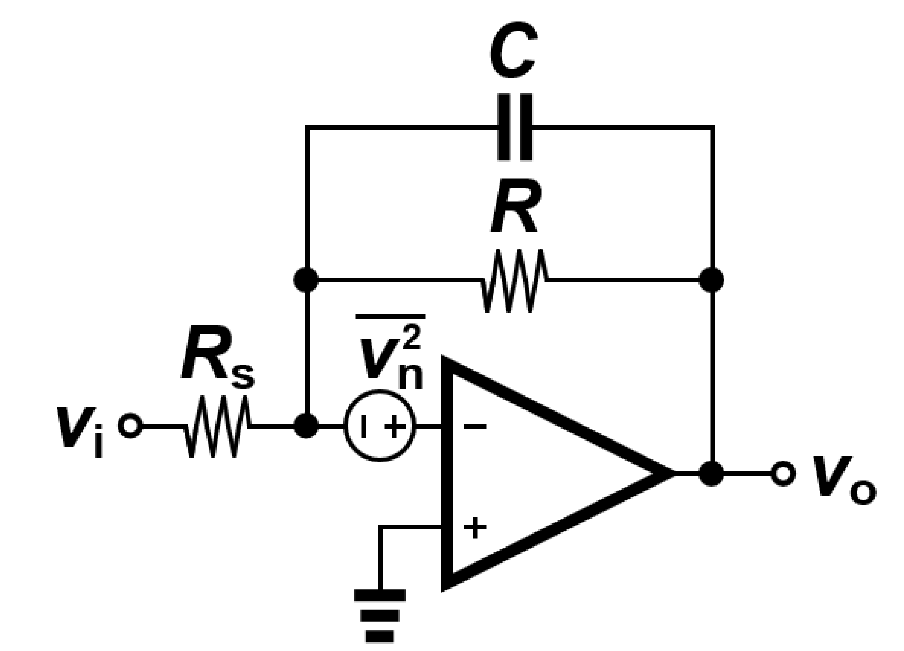
\includegraphics[width=0.4\textwidth]{figs/problem3.png}
\end{figure}

\begin{enumerate}[label=(\alph*)]
  \item {\color{blue}Assume the op-amp has infinite DC gain and infinite GBW ($\omega_u$). Calculate $v_o / v_i$ and total output noise. What issue did you find?}
    \begin{align*}
      \frac{v_o}{v_i} &= \frac{R || C}{R_s} = \frac{\frac{R}{1 + sRC}}{R_s} = \frac{R}{R_s} \frac{1}{1 + sRC} \\
      \overline{v_{n,out,R_s}^2} &= \int_{0}^{\infty} \overline{v_{n,R_s}^2} \left(\frac{v_o}{v_i}\right)^2 df \\
        &= 4kT R_s \left(\frac{R}{R_s}\right)^2 \int_0^{\infty} \left|\frac{1}{1 + sRC}\right|^2 df \\
        &= 4kT R_s \left(\frac{R}{R_s}\right)^2 \frac{1}{4RC}
    \end{align*}
  \item {\color{blue}Assume the op-amp has infinite DC gain and finite GBW (i.e. You can model the op-amp gain $A(s) = -\omega_u/s$ where $\omega_u \gg 1 / RC$). Calculate $v_o/v_i$ and total output noise. How does the noise relate to $\omega_u$?}
\end{enumerate}

\end{document}
